\section{1174054 | Aulyardha Anindita}

\subsection{Teori}
\begin{enumerate}
\item Definisi, Sejarah dan Perkembangan Kecerdasan Buatan
\begin{itemize}
\item Definisi Kecerdasan Buatan\\
Kecerdasan buatan adalah suatu kecerdasan yang didalamnya berisi suatu system yang biasa diatur dalam sebuah konteks ilmiah. Kecerdasan  buatan juga bisa didefinisikan sebagai sebuah kecerdasan yang diciptakan dan dimasukkan kedalam suatu mesin computer agar dapat melakukan pekerjaan seperti yang dapat dilakukan oleh manusia. Ada beberapa macam bidang atau ilmu yang menggunakan kecerdasan buatan diantaranya adalah system pakar, permainan computer (game), logika fuzzy, jaringan saraf tiruan dan robotika.\\
Penelitian dalam AI mencakup pembuatan mesin dan suatu program computer untuk mengotomatisasikan tugas-tugas yang membutuhkan perilaku cerdas, seperti : pengendalian, perencanaan dan penjadwalan serta kemampuan untuk menjawab diagnose dan pertanyaan pelanggan serta pengenalan tulisan tangan. Suara dan wajah

\item Sejarah Kecerdasan Buatan
\begin{itemize}
\item Pada tahun 1940 dan 1950 Artificial Inteligence merupakan suatu inovasi baru dalam bidang ilmu pengetahuan dimana pada tahun ini computer modern sudah ada
\item Pada tahun 1950 awal, studi tentang “mesin berfikir” mempunyai berbegai nama seperti cybernetics, teori automata, dan pemrosesan informasi
\item Pada tahun 1956, para ilmuwan jenius seperti Alan Turing, Norbert, Wiener, Claude Shannon dan Warren McCullough bekerja secara independen di bidang cybernetics, matematika, algoritma dan teori jaringan. John McCarthy merupakan orang yang menciptakan istilah tersebut dan mendirikan laboratorium kecerdasan buatan di MIT dan Stanford
\item Pada tahun 1956, McCarthy mendirikan Konferensi Dartmouth di Hanover, New Hampshire. Dia merupakan peneliti terkemuka dalam teori kompleksitas, simulasi Bahasa, dan hubungan antara keacakan dan pemikiran kreatif, jaringan saraf diundang. Sehingga Konferensi Dartmouth 1956 dianggap sebagai kelahiran Kecerdasan Buatan.
\item Sejak saat itu, Kecerdasan Buatan telah hidup melalui decade kemuliaan dan cemohan yang dikenal dengan luas sebagai musim panas dan musim dingin Ai.
\end{itemize}

\item Perkembangan Kecerdasan Buatan\\
Saat ini, teknologi Artificial Intelligence sangat ramai diperbincangkan oleh masyarakat. Sudah banyak pekerjaan yang hilang karena adanya AI, seperti pekerjaan kasir, penjaga pintu tol, parkir, dan sebagainya. Hal ini terjadi karena AI lebih unggul dalam hal kinerja, fitur dan lain sebagainya. Walaupun masih ada beberapa aspek yang memang pekerja manusia masih unggul dibandingkan AI itu sendiri. \\
Berdasarkan survei yang dilakukan oleh Microsoft, hasilnya adalah 39 responden masih mempertimbangkan untuk menggunakan mobil tanpa pengemudi dan sebanyak 36 responden lainnya setuju mahwa robot atau AI dengan menggunakan software untuk beroperasi mampu meningkatan produktivitas. Dari survei tersebut, dapat ditarik kesimpulan bahwa pengguna AI harus lebih bijaksana dalam pengembangan dan penggunaan dari AI sehingga tidak memiliki efek samping terhadap profuktifitas kerja dan keseharian sebagai pengguna dalam kehidupan sehari-hari.

\end{itemize}

\item Definisi Supervised Learning, Klasifikasi, Regresi, Unsupervised Learning, Data Set, Training Set dan Testing Set
\begin{itemize}
\item Supervised Learning\\
Supervised learning adalah suatu tugas pengumpulan data yang berfungsi untum menyimpulkan fungsi dari data pelatihan yang berlabel. Didalam Supervised Learning, setiap contoh merupakan pasangan yang terdiri dari objek input dan nilai output yang diinginkan. Algoritma pembelajaran yang diawasi berupa menganalisis data pelatihan dan menghasilkan fungsi yang disimpulkan yang digunakan untuk memetakan contoh baru.\\
 	Supervised Learning adalah suatu pendekatan dimana sudah terdapat data yang dilatih selain itu juga sudah memiliki variable yang ditargetkan sehingga tujuan dari pendekatan tersebut adalah mengelompokkan suatu data ke data yang sudah ada. Supervised learning sendiri menyediakan algoritma pembelajaran dengan jumlah yang diketahui untuk mendukung penilaian dimasa depan. Supervised learning sebagian besar memiliki kaitan dengan AI dengan menggunakan model pembelajaran generatif. Data pelatihan untuk pembelajaran yang diawasi mencakup beberapa contoh dengan subjek input yang berpasangan dan output yang diinginkan.\\
 	Modul supervised learning mempunyai beberapa keunggulan dibandingkan pendekatan tanpa pengawasan, tapi mereka juga memiliki keterbatasan. System lebih cenderung membuat penilaian bahwa manusia dapat berhubungan, misalnya manusia mempunyai dasar untuk keputusan. Tapi, dalam kasus tersebut yang menggunakan metode berbasis pengambilan, supervised learning mengalami kseulitan dalam menangani suatu informasi baru. 

\item Klasifikasi\\
Klasifikasi merupakan pembagian menurut kelas-kelas. Menurut ilmu pengetahuan, klasifikasi adalah suatu proses pengelompokkan benda berdasarkan ciri-ciri persamaan dan perbedaan. Dalam pembelajaran mesin dan statistic, klasifikasi merupakan suatu pendekatan pembelajaran yang diawasi dimana program computer tersebut belajar dari input data yang diberkan kepadanya lalu menggunakan pembelajaran tersebut untuk mengklasifikasikan pengamatan baru. Kumpulan data tersebut mungkin hanya bersifat dua kelas atau mungkin juga multi-kelas.

\item Regresi\\
Regresi adalah suatu metode analisis statistik yang digunakan untuk melihat pengaruh antara dua atau lebih variable. Regresi sendiri membahas masalah ketika variable output yaitu nilai ril atau berkelanjutan seperti gaji atau berat. Banyak model yang dapat digunakan, yang paling sederhana adalah regresi linear.

\item Unsupervised Learning\\
Unsupervised learning berbeda dengan supervised learning, perbedaanya yaitu unsupervised learning tidak memiliki data pelatihan, sehingga data dapat dikelompokkan menjadi dua atau 3 begitupun seterusnya. Unsupervised learning adalah suatu pelatihan algoritma kecerdasan buatan (AI) menggunakan beberapa informasi yang tidak diklasifikasikan atau diberi label dan memungkinkan algoritma  untuk bertindak atas informasi tersebut. System AI disini dapat dikelompokkan berdasarkan informasi yang tidak disortir berdasarkan persamaan dan perbedaan meskipun tidak ada kategori yang disediakan. System AI disajikan dengan data yang tidak berlabel, tidak terkategorisasi dan algoritma system bekerja pada data tanpa pelatihan sebelumnya sehingga outputmya tergantung pada algoritma kode.

\item Data Set\\
Data set adalah suatu objek yang merepresentasikan data dan memiliki relasi yang ada di dalam memory. Struktur data set mirip dengan data yang ada didatabase, namun bedanya data set berisi koleksi dari data table dan data relation. Untuk mendapatkan data yang tepat, berarti mengumpulkan atau mengidentifikasi data yang berkorelasi dengan hasil yang ingin anda prediksi.

\item Training Set\\
Training set adalah salah satu set yang biasa digunakan oleh algoritma klasifikasi. Seperti decision tree, bayesian, neural network, dll. Mereka dapat digunakan untuk membentuk model classifier, dalam menjalankan pelatihan yang diatur melalui jaringan saraf yang mengajarkan pada net dengan cara menimbang berbagai fitur, menyesuaikan koefisien berdasarkan kemungkinan mereka meminimalkan kesalahan. Kofiesen tersebut juga dikenal sebagai parameter.

\item Testing Set\\
Testing set adalah salah satu set yang digunakan untuk mengukur sejauh mana classifier berhasil melakukan klasifikasi dengan benar. Hal ini berfungsi sebagai materai persetujuan tapi tak digunakan sampai akhir. Setelah melatih dan mengoptimalkan data, kita dapat melakukan pengujian sarat terhadap pengambilan sampel aca. Dan hasilnya harus memvalidasi bahwa jaring data tersebut secara akurat mengenali gambar atau mengenali setidaknya (x) dari jumlah tersebut.

\end{itemize}
\end{enumerate}

\subsection{Praktek}
\begin{enumerate}
\item Instalasi library scikit dari anaconda
\hfill\break
	\begin{figure}[H]
		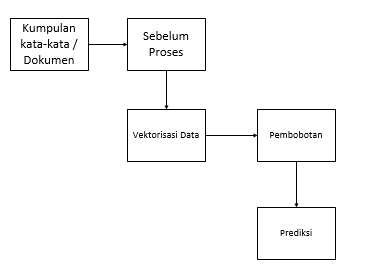
\includegraphics[width=4cm]{figures/1174054/1/1.png}
		\centering
		\caption{Instalasi Package Scikit Learn}
	\end{figure}
	\begin{figure}[H]
		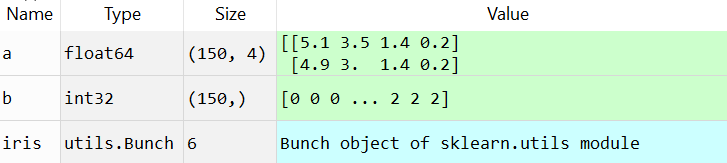
\includegraphics[width=4cm]{figures/1174054/1/2.png}
		\centering
		\caption{Isi Variabel Explorer}
	\end{figure}
\item Mencoba Loading an example dataset
\hfill\break
	\lstinputlisting[firstline=8, lastline=12]{src/1174054/1/1174054.py}
	
\item Mencoba Learning and predicting
\hfill\break
	\lstinputlisting[firstline=14, lastline=24]{src/1174054/1/1174054.py}
	
\item Mencoba Model persistence
\hfill\break
	\lstinputlisting[firstline=26, lastline=36]{src/1174054/1/1174054.py}
	
\item Mencoba Conventions
\hfill\break
	\lstinputlisting[firstline=38, lastline=50]{src/1174054/1/1174054.py}
\end{enumerate}

\subsection{Penanganan Error}
\begin{enumerate}
\item ScreenShoot Error
	\begin{figure}[H]
		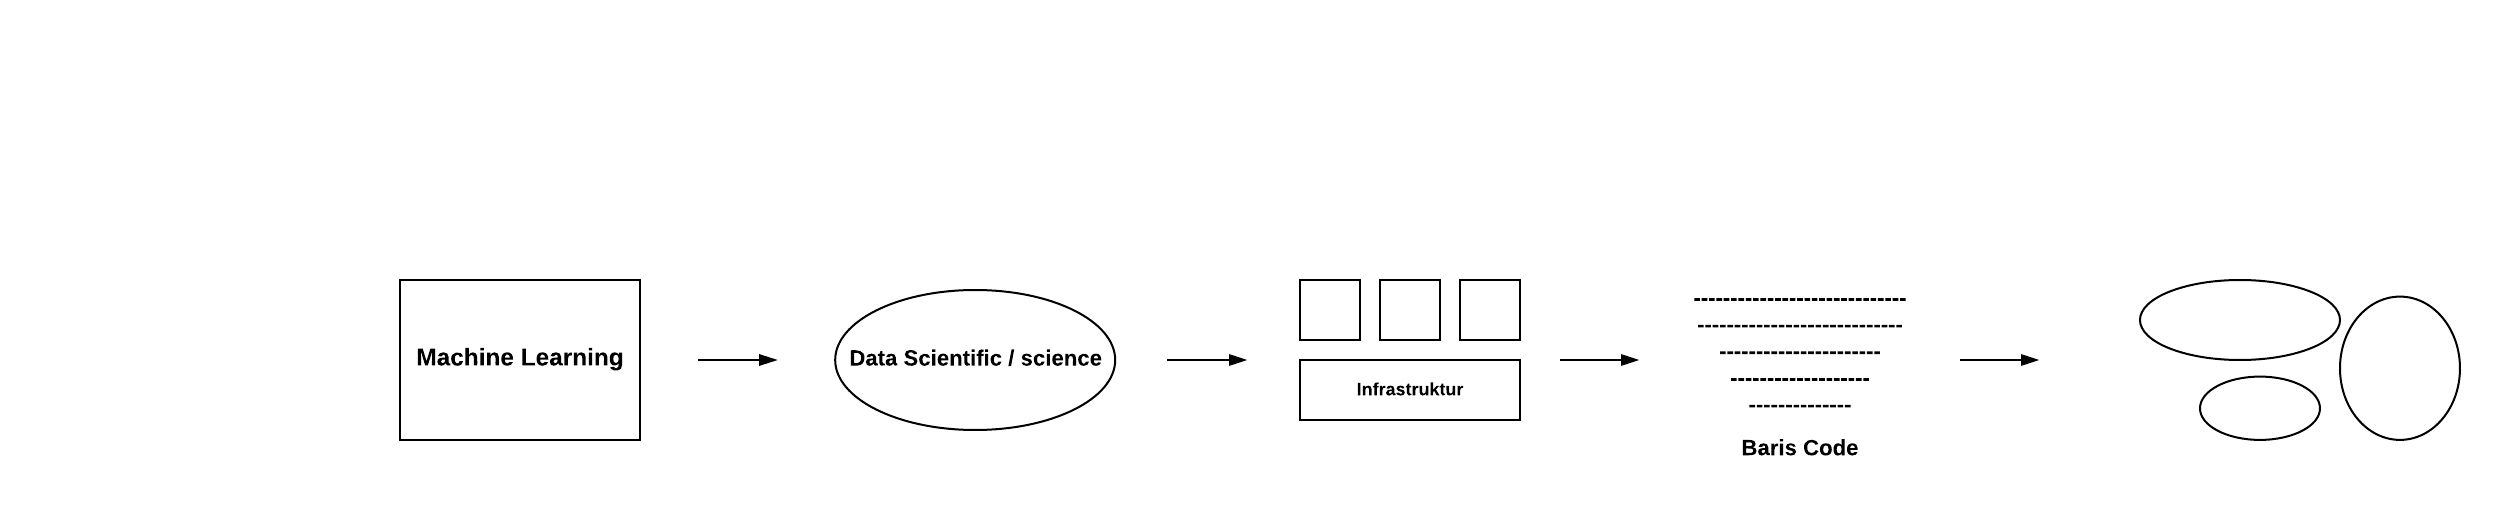
\includegraphics[width=4cm]{figures/1174054/1/3.png}
		\centering
		\caption{Module Not Found Error}
	\end{figure}
	\begin{figure}[H]
		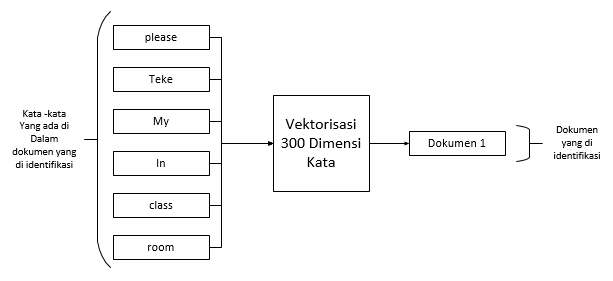
\includegraphics[width=4cm]{figures/1174054/1/4.png}
		\centering
		\caption{Import Error}
	\end{figure}

	\item Tuliskan Kode Error dan Jenis Error
	\begin{itemize}
		\item Module Not Found Error
		\item Import Error
	\end{itemize}
	\item Cara Penanganan Error
	\begin{itemize}
		\item Module Not Found Error
		\hfill\break
		Dengan memperbaiki penulisan atau kesalahan dalam penulisan kode atau melakukan install package atau modul yang belum terinstal
		\item Import Error
		\hfill\break
		Dengan Menginstall Library Yang Tidak Ditemukan
	\end{itemize}
\end{enumerate}


\subsection{Bukti Tidak Plagiat}
\begin{figure}[H]
	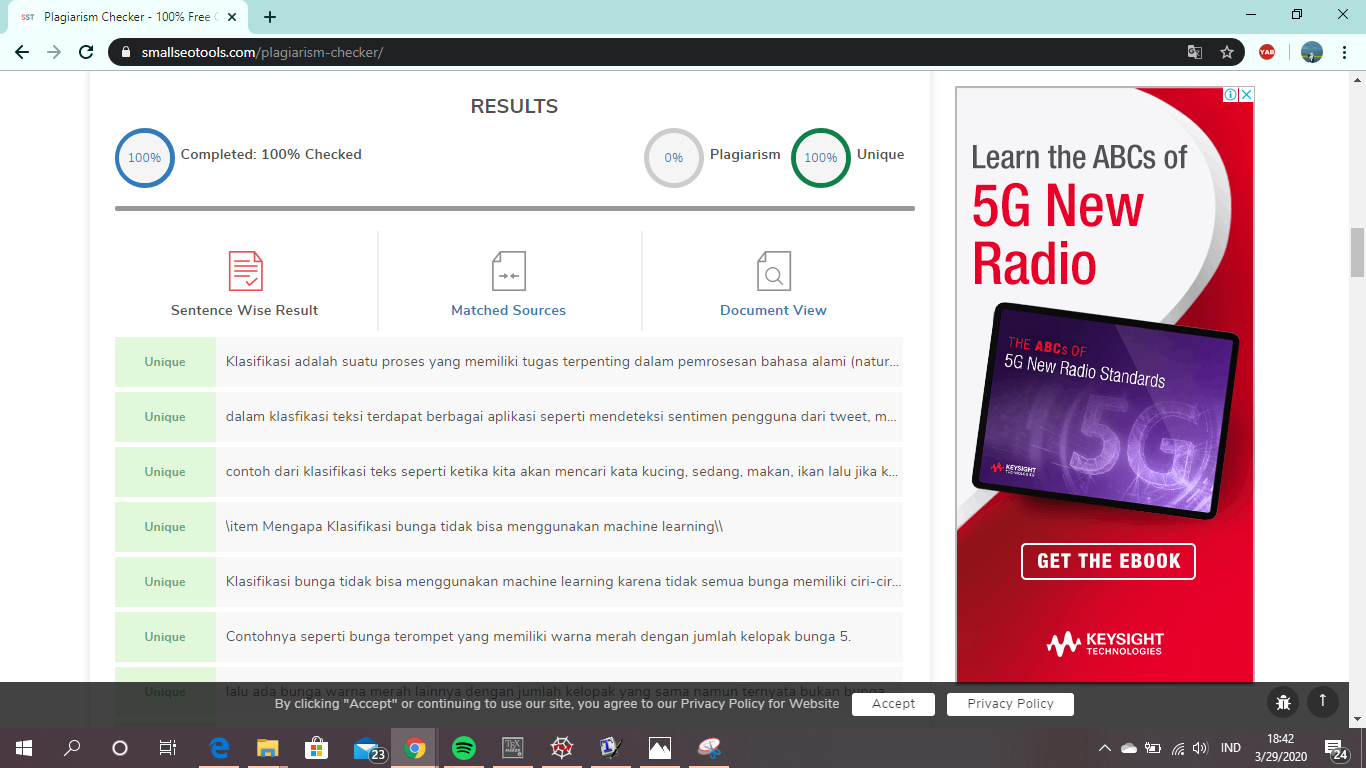
\includegraphics[width=4cm]{figures/1174054/1/plagiarisme.png}
	\centering
	\caption{Bukti Plagiasrisme}
\end{figure}

\subsection{Link Youtube}
https://youtu.be/gl9Q60DzEfI